\documentclass[a4paper,10pt]{memoir}
\usepackage[italian]{babel}
\usepackage{wrapfig}
\usepackage[pdftex]{graphicx}
\usepackage{graphviz}
\usepackage{graphicx}
\usepackage{amsmath}
\usepackage{float}

%Define the listing package
\usepackage{listings} %code highlighter
\usepackage{color} %use color
\definecolor{mygreen}{rgb}{0,0.6,0}
\definecolor{mygray}{rgb}{0.5,0.5,0.5}
\definecolor{mymauve}{rgb}{0.58,0,0.82}
 
%Customize a bit the look
\lstset{ %
backgroundcolor=\color{white}, % choose the background color; you must add \usepackage{color} or \usepackage{xcolor}
basicstyle=\footnotesize, % the size of the fonts that are used for the code
breakatwhitespace=false, % sets if automatic breaks should only happen at whitespace
breaklines=true, % sets automatic line breaking
captionpos=b, % sets the caption-position to bottom
commentstyle=\color{mygreen}, % comment style
deletekeywords={...}, % if you want to delete keywords from the given language
escapeinside={\%*}{*)}, % if you want to add LaTeX within your code
extendedchars=true, % lets you use non-ASCII characters; for 8-bits encodings only, does not work with UTF-8
frame=single, % adds a frame around the code
keepspaces=true, % keeps spaces in text, useful for keeping indentation of code (possibly needs columns=flexible)
keywordstyle=\color{blue}, % keyword style
% language=Octave, % the language of the code
morekeywords={*,...}, % if you want to add more keywords to the set
numbers=left, % where to put the line-numbers; possible values are (none, left, right)
numbersep=5pt, % how far the line-numbers are from the code
numberstyle=\tiny\color{mygray}, % the style that is used for the line-numbers
rulecolor=\color{black}, % if not set, the frame-color may be changed on line-breaks within not-black text (e.g. comments (green here))
showspaces=false, % show spaces everywhere adding particular underscores; it overrides 'showstringspaces'
showstringspaces=false, % underline spaces within strings only
showtabs=false, % show tabs within strings adding particular underscores
stepnumber=1, % the step between two line-numbers. If it's 1, each line will be numbered
stringstyle=\color{mymauve}, % string literal style
tabsize=2, % sets default tabsize to 2 spaces
title=\lstname % show the filename of files included with \lstinputlisting; also try caption instead of title
}
%END of listing package%
 
\definecolor{darkgray}{rgb}{.4,.4,.4}
\definecolor{purple}{rgb}{0.65, 0.12, 0.82}
 
%define Javascript language
\lstdefinelanguage{JavaScript}{
keywords={typeof, new, true, false, catch, function, return, null, catch, switch, var, if, in, while, do, else, case, break},
keywordstyle=\color{blue}\bfseries,
ndkeywords={class, export, boolean, throw, implements, import, this},
ndkeywordstyle=\color{darkgray}\bfseries,
identifierstyle=\color{black},
sensitive=false,
comment=[l]{//},
morecomment=[s]{/*}{*/},
commentstyle=\color{purple}\ttfamily,
stringstyle=\color{red}\ttfamily,
morestring=[b]',
morestring=[b]"
}
 
\lstset{
language=JavaScript,
extendedchars=true,
basicstyle=\footnotesize\ttfamily,
showstringspaces=false,
showspaces=false,
numbers=left,
numberstyle=\footnotesize,
numbersep=9pt,
tabsize=2,
breaklines=true,
showtabs=false,
captionpos=b
}

\usepackage[chapter]{minted}
\usepackage{adjustbox}
\usepackage{hyperref}
\hypersetup{
  colorlinks   = true,    % Colours links instead of ugly boxes
  urlcolor     = black,    % Colour for external hyperlinks
  linkcolor    = black,    % Colour of internal links
  citecolor    = black      % Colour of citations
}

% import package
\usepackage{FrontespizioSapienza}

\pagestyle{plain}%%to insert the number of the page

% declare info
\FSSTitolo{Titolo}
\FSSFacolta{Ingegneria dell'Informazione, Informatica e Statistica}
\FSSCorso{Informatica}

\FSSCandidato{Edoardo Ottavianelli}
\FSSMatricola{1756005}
\FSSRelatore{Emanuele Panizzi}
\FSSCorrelatore{}
\FSSAnnoAccademico{2019/2020}


\begin{document}

\frontmatter


% print title
\maketitle
\cleardoublepage

%\vspace*{10cm}
%\begin{flushright}
%\textsl{...}
%\end{flushright}
%\cleardoublepage

% ======================================= ABSTRACT ================================================
\begin{abstract}
  abstract
\end{abstract}
\cleardoublepage

\tableofcontents
\cleardoublepage

\mainmatter

\renewcommand\chapterheadstart{}
\renewcommand\printchaptername{}
\renewcommand\chapternamenum{}
\renewcommand\printchapternum{}
\renewcommand\afterchapternum{}
\renewcommand\printchaptertitle[1]{\chaptitlefont \thechapter. \space #1}


% ======================================= CHAPTER 1 ================================================
\chapter{Introduzione a SeismoCloud e obiettivi del progetto}

\section{I terremoti e la loro natura}

\begin{wrapfigure}[14]{r}{0.50\textwidth}
\caption{Composizione della Terra}
\label{fig:crostaterrestre}
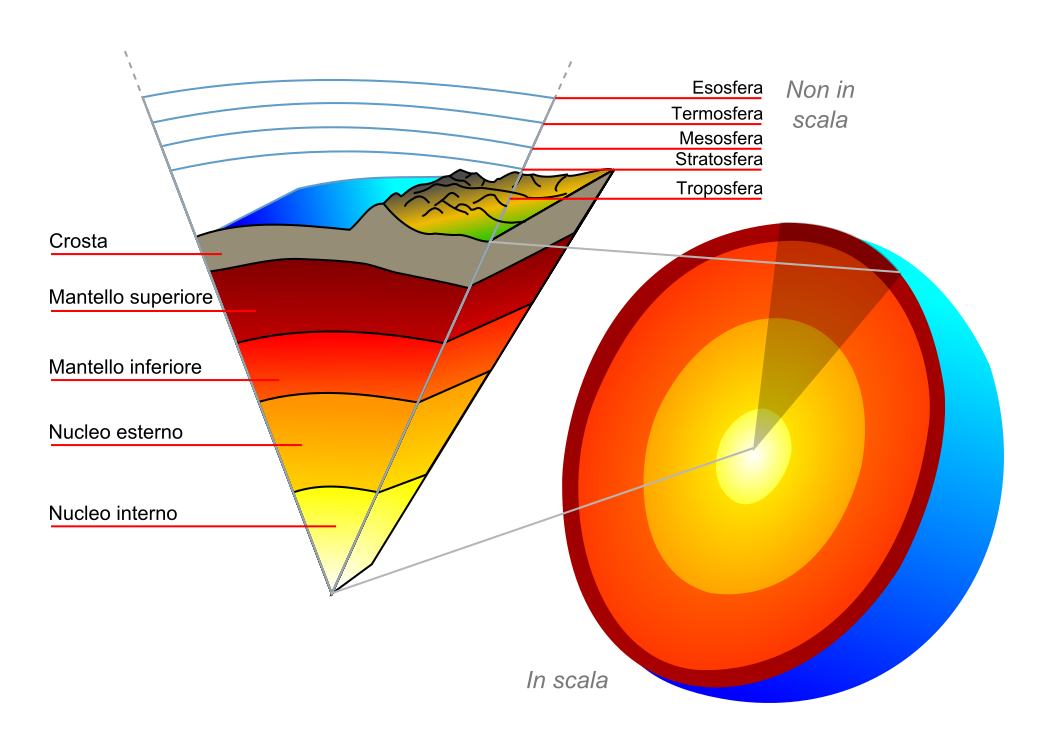
\includegraphics[width=0.50\textwidth]{Chapter-1/crosta-terrestre.png}
\end{wrapfigure}

La terra è composta a strati, o meglio da involucri concentrici (Figura 1.1 a lato) ed ognuno di essi ha diverse caratteristiche e particolarità.
Al centro della Terra c'è il \textbf{nucleo interno}, ossia un ammasso viscoso composto quasi esclusivamente da ferro avente un raggio di circa 1250 km. Si raggiungono temperature molto elevate, circa 5000-6000$^{\circ}$C.
A seguire abbiamo il \textbf{nucleo esterno}, principalmente composto per il 20\% da ferro e la restante parte nichel, raggiunge circa i 3000$^{\circ}$C. Comprendendo anche il nucleo interno, ha un raggio di circa 3500 km.

Continuando verso l'esterno, troviamo il \textbf{mantello terrestre}, che si divide in superiore ed inferiore.
\\
È composto da diversi metalli ed è difficile stabilire la temperatura dato i moti convettivi del calore, ma si stima intorno ai 500$^{\circ}$C a confine con la crosta terrestre e 3000$^{\circ}$C a confine con il nucleo.
\\
Infine abbiamo la \textbf{crosta terrestre}, che partendo dalla superficie, arriva fino a 70 km di profondità.
\\
Insieme, il \textit{mantello superiore} e la \textit{crosta terrestre} formano la \textbf{litosfera}.
La litosfera è suddivisa in una decina di placche tettoniche principali e altre numerose placche di minori dimensioni (figura 1.2). Queste placche "galleggiano" sullo strato immediatamente sottostante del mantello superiore.
\\
Esse, data la forte pressione e le alte temperature, subiscono sforzi di enormi dimensioni che formano i \textbf{terremoti}.
\\
I terremoti sono vibrazioni della crosta terrestre, provocate dallo spostamento  di una o più placche nella litosfera.
Le placche si muovono flettendosi lentamente e poi rilasciando (raggiunto il \textit{punto di rottura}) in maniera elastica tutta l'energia accumulata.
Il punto in cui viene generata questa energia è detto \textbf{ipocentro}, zona in cui sono presenti delle fratture chiamate \textit{faglie}, mentre il punto in superficie posto sulla verticale dell'ipocentro è chiamato \textbf{epicentro}.
\clearpage


\begin{figure}
\caption{Placche tettoniche}
\label{fig:placchetettoniche}
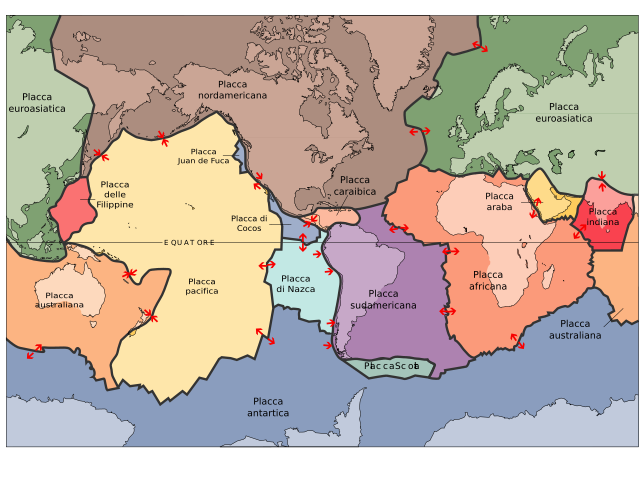
\includegraphics[width=1\textwidth]{Chapter-1/placche-tettoniche.png}
\end{figure}

Esistono tre tipi di faglie: faglie \textit{trascorrenti}, faglie \textit{dirette} e \textit{inverse}.
Esistono in egual numero differenti tipi di onde sismiche.
\\
Le \textbf{onde di compressione o longitudinali} fanno comprimere e dilatare la materia nella stessa direzione con cui si propaga l'onda.
Sono anche dette \textit{primarie}, perché sono le onde che viaggiano a velocità più elevate.
\\
Le \textbf{onde di taglio o trasversali} fanno compiere alla materia oscillazioni in modo perpendicolare alla loro direzione di propagazione. Hanno effetto solo nei solidi, non possono propagarsi attraverso corpi liquidi o gassosi.
Vengono chiamate anche \textit{onde secondarie}, essendo meno veloci delle precedenti.
\\
Le \textbf{onde superficiali}, anche se il nome può essere mal interpretato, non si manifestano in superficie. Questo tipo di onde sono la combinazione delle due precedenti, perciò sono molto complesse e sono le più pericolose. 

\clearpage

\section{Misurazione dei terremoti}

\subsection{Tipologie di terremoti}
Abbiamo 4 differenti tipologie di terremoti: \textit{tettonici}, \textit{vulcanici}, \textit{da crollo} e \textit{artificiali}.
\\
I terremoti \textbf{tettonici}, come dice il nome, sono provocati dal movimento delle placche tettoniche e hanno origine lungo le faglie.
Sono i più pericolosi ed i più frequenti.
\\
I terremoti \textbf{vulcanici} sono originati dall'attività vulcanica nel sottosuolo. Sono meno pericolosi dei precedenti data la minor energia rilasciata e l'estensione limitata.
\\
I terremoti \textbf{da crollo} si originano durante il crollo di montagne, grotte o frane. Hanno una bassa pericolosità e frequenza.
\\
Infine, i terremoti \textbf{artificiali} vengono originati da attività umane. Ad esempio, una grande esplosione. In generale, hanno una potenza molto limitata.


\subsection{Metodologie di misurazione}
Esistono due tipologie principali di misurazione di un terremoto: la scala \textbf{Mercalli} e la scala \textbf{Richter}.
\\
La scala Mercalli misura l'\textit{intensità} di un terremoto osservando i danni causati da esso. Per questo, dato che tiene in conto solo degli effetti che la scossa produce, può essere applicata anche ai terremoti avvenuti nel passato.
Assegna dei numeri crescenti per intensità, si va dall'uno (impercettebile) sino a dodici (apocalittica).
\\
La scala (o meglio \textit{indice}) Richter misura invece l'energia sprigionata dalla scossa, ossia la \textit{magnitudo}. Viene chiamata scala, ma è più corretto dire indice dato che non ha un range di valori finito. La magnitudo è descritta da questa formula:

\begin{equation*}
  M_w = {\frac{2}{3}}\log_{10}(M_\mathrm{0}) - 6
\end{equation*}
\\
dove $M_0$ è il momento sismico all'ipocentro da esprimere in Newton per metro|N·m.
\\
Ad oggi il massimo valore magnitudo registrato è 9,5.
\\
\subsection{Strumenti di misurazione}
Sono principalmente due: il \textbf{sismografo} ed il \textbf{sismometro}.
\\
Entrambi misurano accelerazione e velocità dei movimenti del suolo, con la differenza che il sismometro misura solamente, ma non può registrare i dati; il sismografo invece oltre alla misura produce anche un grafico temporale, chiamato appunto \textit{sismogramma}.
\\
Quella che vediamo in Figura 1.3 è la \textbf{Rete Sismica Nazionale}.
\\
È una rete di stazioni sismiche (circa 300) disposte su tutto il territorio italiano e appena fuori dai confini.
Per la maggioranza sono stazioni dell'INGV (Istituto Nazionale di Geologia e Vulcanologia), ma ne fanno parte anche altre piccole reti.
\\
Questa rete monitora sette giorni su sette, 24 ore su 24 i movimenti del suolo e li registra, inviandoli poi ai centri di elaborazione dati di Roma, Grottaminarda e Catania.
\\
La concentrazione maggiore di terremoti in Italia è nell'appennino e nel sud Italia, per questo la maggior parte delle stazioni è posizionata in questi punti.

\clearpage

\begin{figure}
\caption{Rete Sismica Nazionale}
\label{fig:RSN}
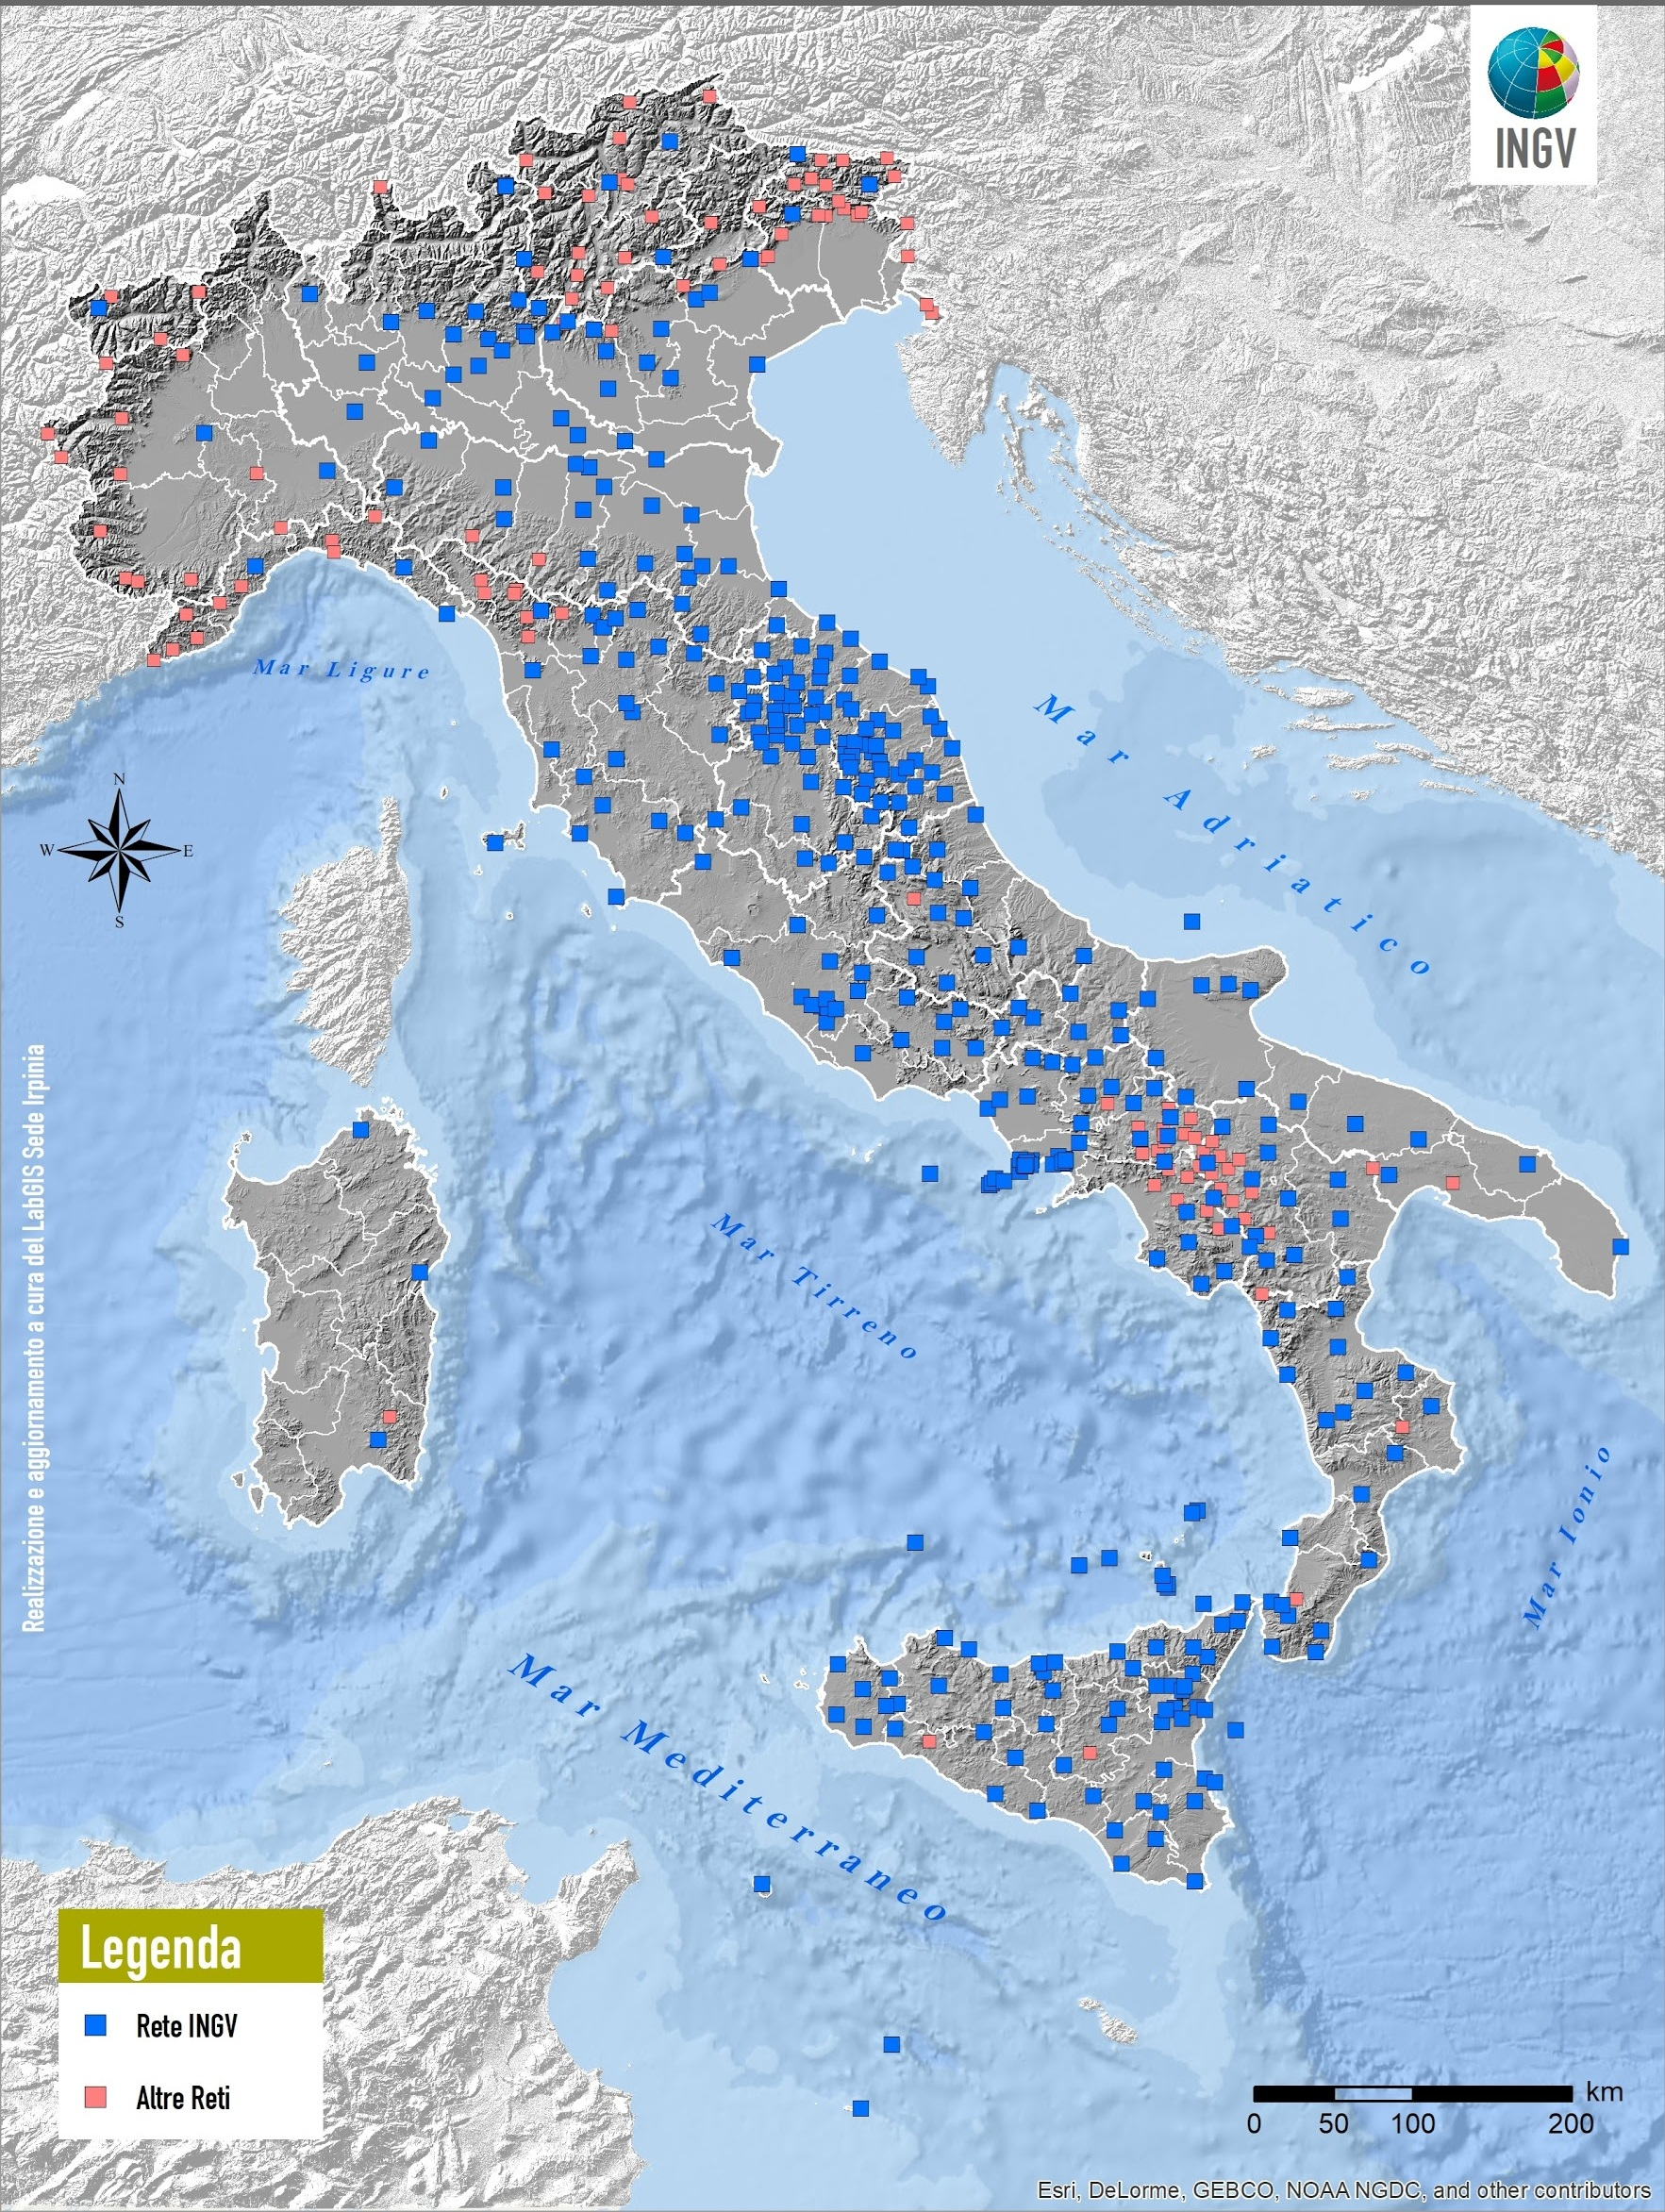
\includegraphics[width=1\textwidth]{Chapter-1/RSN.jpg}
\end{figure}

\clearpage

\section{Piattaforma SeismoCloud}

\subsection{Introduzione al progetto}

\begin{wrapfigure}[14]{r}{0.15\textwidth}

\includegraphics[width=0.15\textwidth]{Chapter-1/seismocloud.png}

\includegraphics[width=0.15\textwidth]{Chapter-1/ingv.jpg}
\end{wrapfigure}

SeismoCloud è una rete di sismometri a basso costo distribuiti in tutta Italia. 
Ha come scopo l'\textit{Earthquake Early Warning}, ossia monitorare l'attività sismica e, nel caso viene rilevato un terremoto, notificare le persone interessate.
\\
L'obiettivo specifico dell'EEW è l'avviso \textbf{in tempo reale} di un possibile sisma.
\\
I sismometri possono essere costruiti personalmente se si ha capacità di elettronica di base, altrimenti viene utilizzato il sensore interno di uno smartphone.
\\
È un progetto nato dall'Università La Sapienza e l'INGV.

\subsection{Architettura di sistema}
I sismometri sono di due tipologie: \textit{fissi} e \textit{mobili}.
\\
I \textbf{sismometri fissi} sono dei componenti elettronici formati da un chip a basso costo con un modulo Wi-Fi integrato per la connessione ad Internet e un modulo con giroscopio e accelerometro.
Per una migliore rilevazione si consiglia di fissarli ad un muro.
\\
I \textbf{sismometri mobili} invece utilizzano l'applicazione per smartphone, abilitando l'accelerometro interno del telefono per rilevare vibrazioni.
\\
Devono essere appoggiati su un piano, per esempio un tavolo.
\\
Durante la registrazione di un nuovo sismometro, esso viene localizzato per conoscere la sua posizione (fondamentale al rilevamento corretto dei sismi). Nonostante ciò la privacy può essere conservata mostrando il sismometro nella mappa pubblica con una finta posizione casuale nel raggio di 2km.
\\
I sismometri utilizzano il protocollo ISO standard \textbf{MQTT} (Message Queue Telemetry Transport) per inviare e ricevere messaggi.
\\
È stato progettato per un basso impatto a livello di banda e di risorse. I client si iscrivono ad un \textit{topic}, ossia un identificatore che si riferisce ad un dato ben preciso (ad esempio \textit{sensor/temperature}).
\\
Oltre a ricevere dati, posso \textit{pubblicarli}, cioè inviare dati riferiti ad un topic, dati che gli iscritti al topic riceveranno. 
I dati inviati vengono elaborati in un server centrale che li gestisce, compie dei calcoli su di essi e li archivia.\\

\begin{figure}[H]
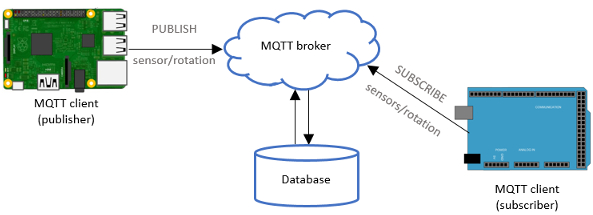
\includegraphics[width=1\textwidth]{Chapter-1/mqtt.jpg}
\end{figure}

\clearpage


Per i messaggi di invio e ricezione dei sismometri e per tutti i dati prodotti da essi viene utilizzato lo stile architetturale \textbf{REST} (REpresentational State Transfer).
\\
Questo schema è definito da dei principi: 
\begin{itemize}
  \item Tutto è considerato una risorsa
  \item Ogni risorsa è identificabile da un URI (Uniform Resource Identifier)
  \item Usa metodi HTTP standard (GET, POST, PUT, DELETE)
  \item Possibili rappresentazioni multiple per la stessa risorsa
  \item La comunicazione deve essere sempre senza stato
\end{itemize}
Un esempio di risorsa in stile REST è: \textit{example.domain/sensor/sensor-id/connect}, dove sensor-id è l'identificatore unico per un sensore.
\\
Tramite l'app mobile (disponibile per Android e iOS) è possibile visualizzare la lista dei propri sismometri, una mappa aggiornata in tempo reale con i sismometri attivi e i terremoti recenti, una lista di terremoti con relativa magnitudo, posizione e profondità dell'ipocentro (ordinati cronologicamente) e infine alcuni informazioni utili.
\\
Tramite l'interfaccia web è possibile visualizzare tutte le informazioni prima citate ed in più una dashboard personalizzata (\href{https://my.seismocloud.com}{my.SeismoCloud.com}).
Nella dashboard personale è possibile visualizzare due grafici che mostrano il tempo di utilizzo assoluto e settimanale di ogni sismometro attivo.
\\
Dopo l'effettiva autenticazione (tramite password o QRCode) si entra nella parte privata, ossia relativa ad un determinato \textit{gruppo} (insiemi di sismometri raggruppati per locazione).
\\
Qui, oltre alle funzionalità citate, è presente un sistema di \textbf{EUD} (End User Development).
\\
È un sistema che permette agli utenti di programmare delle azioni e svolgere dei compiti quando si verificano opportune condizioni.
\\
Ad esempio, si può ricevere un messaggio automatico tramite Telegram ogni volta che il mio sismometro vibra.

\begin{figure}
\caption{Achitettura di SeismoCloud}
\label{fig:ArchitetturaSeismoCloud}
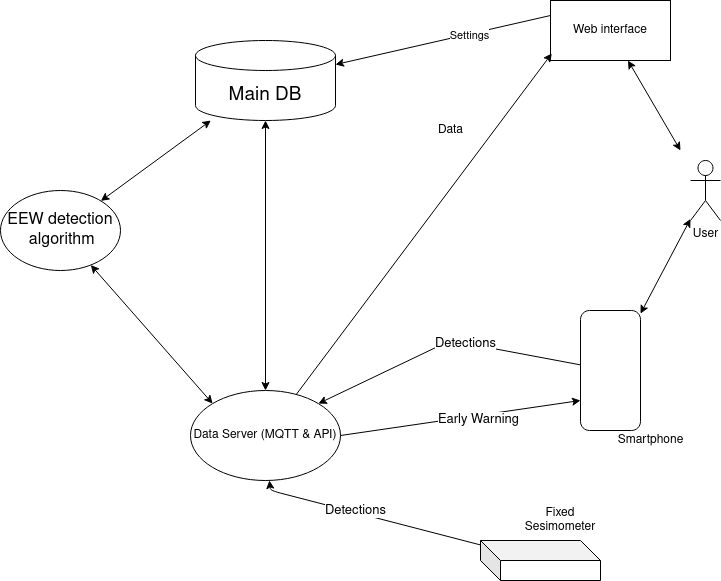
\includegraphics[width=1\textwidth]{Chapter-1/architettura-seismocloud.png}
\end{figure}

\clearpage

\section{Community SeismoCloud}

\subsection{Un lavoro di gruppo}

\begin{wrapfigure}[14]{r}{0.55\textwidth}
\caption{Rete Sismica SeismoCloud}
\label{fig:RSS}
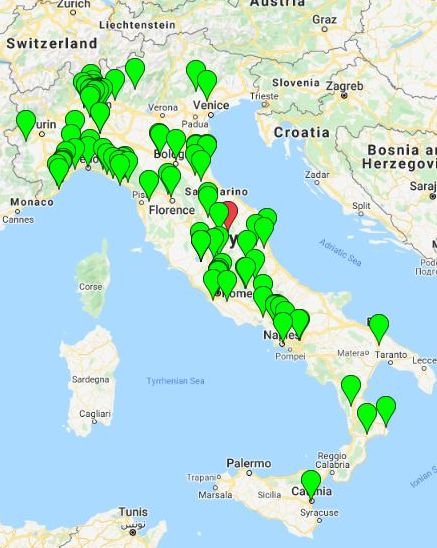
\includegraphics[width=0.55\textwidth]{Chapter-1/seismoitalia.jpg}
\end{wrapfigure}
Come si può notare dalla Figura 1.5 (a lato) la \textbf{Rete Sismica SeismoCloud} si estende su tutto il territorio nazionale. Si contano circa 100 sismometri attivi.\\
Ad oggi il sistema EEW non è attivo perché i sismometri presenti non bastano a compiere delle rilevazioni sufficienti.\\
I nodi della rete sono ben distribuiti nel centro Italia, poco nel Sud. Questo è un problema perché l'attività sismica principale in Italia si sviluppa lungo la catena appenninica fino in Sicilia. \\
Grande menzione meritano anche i \\vulcani attivi (Etna, Stromboli, Vesuvio, \\Vulcano).\\ La community è attiva su vari canali: \\un gruppo su Telegram ed uno su \\Facebook.\\
Il codice di alcune porzioni di sistema \\è disponibili su GitHub sotto
\\
l'organizzazione \href{https://github.com/SapienzaApps}{SapienzaApps}.\\
SeismoCloud viene presentato anche nelle \\scuole per sensibilizzare gli studenti \\sul tema terremoti ed
utilizzare \\questo progetto come
strumento didattico.

\subsection{Bisogni della community}

Attivando un sismometro produco una mole abbastanza consistente di dati.\\
Con una cadenza periodica (qualche minuto, dipende dal carico del sistema) vengono pubblicati questi dati: indirizzo IP locale e pubblico, indirizzo MAC e qualità del segnale della rete Wi-Fi, localizzazione e temperatura del sismometro, soglia attuale (valore utile alla rilevazione di una vibrazione).\\
Quando il sismometro rileva una vibrazione viene inviata l'intensità della vibrazione.\\
Un topic MQTT è dedicato al comando \textit{reboot}, ossia la possibilità di riavviare il sismometro pubblicando un messaggio.\\
Come è stato accennato nella descrizione dell'architettura del sistema (Cap 1.3), è possibile programmare della azioni quando si verificano determinate condizioni.\\
Sostanzialmente le condizioni sono due: quando n sismometri vibrano/sono accesi, oppure la notifica di un Earthquake Early Warning.
Le possibilità per il metodo di notifica sono quattro: un messaggio tramite Telegram, una notifica push ai membri del gruppo, un widget e la pubblicazione di una API.\\

\begin{figure}[H]
\caption{Vecchio sistema EUD}
\label{VecchioEUD}
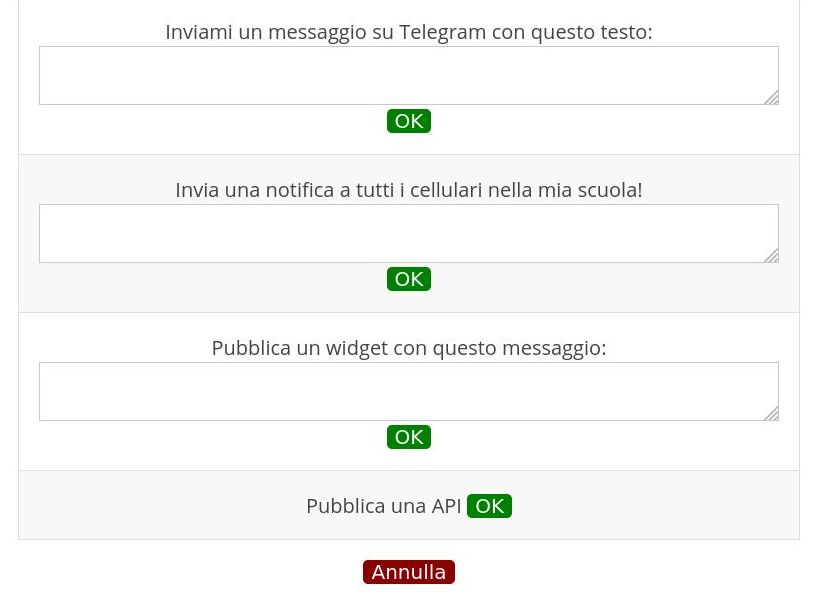
\includegraphics[width=1\textwidth]{Chapter-1/eud-vecchio.jpg}
\end{figure}

Visto che i dati prodotti sono tanti, sarebbe molto utile ampliare il range di condizioni ad un più vasto campo, tenendo in conto anche di tutti i dati che non vengono considerati in questo sistema.\\
Sarebbe molto più utile lasciare completa \textbf{libertà all'utente} (sotto alcune restrizioni di sicurezza) integrando il sismometro con l'ambiente locale. 
\\
Ad esempio una casa smart con dispositivi IoT o altre tipologie di interazione. 
\\
Potrei quindi decidere di riavviare il mio sismometro ogni volta che la temperatura supera i 50$^{\circ}$C. Oppure mandare una mail, pubblicare un tweet e scaricare un file quando vengono rilevate tre vibrazioni nello stesso minuto.
\\
Il tutto non deve risultare complesso, deve essere possibile l'utilizzo per utenti non esperti in informatica o elettronica, ma allo stesso tempo i più competenti devono poter sfruttare le loro abilità.
\\
La soluzione a questo bisogno dovrebbe essere: \textit{facilmente utilizzabile, sicura, affidabile e performante}.
\clearpage

% ======================================= CHAPTER 2 ================================================
\chapter{Architettura del sistema}

\section{Perché Node-RED}

\subsection{Candidati iniziali}

Piuttosto che progettare e costruire uno strumento di End User Development da zero, si è cercato uno scheletro già pronto e maturo. La ricerca è stata piuttosto semplice, un po' meno la valutazione dei possibili candidati.
\\
Il primo candidato è \textbf{IFTTT} (\href{https://iftt.com}{https://ifttt.com}). È lo strumento più famoso, utilizzato da molte persone, con più di 5 milioni di download su Play Store. Il vantaggio di questa scelta è sicuramente la grande maturità della piattaforma. Gli svantaggi sono la difficoltà nell'integrare i nostri dispositivi con questo sistema, ma soprattutto la somiglianza con il sistema EUD da rimpiazzare, troppo semplice e con condizioni e azioni predefinite.
\\
Una seconda scelta è \textbf{draw.io} (\href{https://app.diagrams.net/}{https://draw.io}). Strumento completamente differente al precedente, è un creatore di diagrammi di flusso. Questo è un tipo di programmazione di azioni che lascia molta libertà all'utente, rimanendo semplice ma efficace. 
\begin{figure}[H]
\caption{Esempio di flusso esportato da draw.io}
\label{fig:drawio}
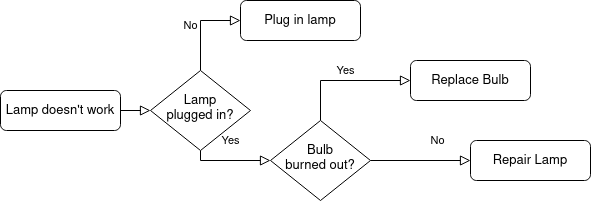
\includegraphics[width=1\textwidth]{relazione-tirocinio/Chapter-2/drawio.png}
\end{figure}
Il codice sorgente di draw.io è disponibile su GitHub. È  ben documentato, quindi questo aiuta l'integrazione con SeismoCloud. Purtroppo si tratta di uno strumento front-end, quindi manca tutta la logica back-end; i dati inseriti dall'utente vengono esportati in file di tipo xml che devono poi essere tradotti in azioni registrate dal sistema. 
\\

\subsection{Scelta Node-RED}
Lo strumento che risolve i problemi precedentemente elencati è \textbf{Node-RED} (\href{https://nodered.org}{https://nodered.org}).
Come draw.io è un creatore di diagrammi di flusso ed è anche open-source con repository su GitHub sotto l'organizzazione \href{https://github.com/node-red}{node-red}. È un servizio orientato all'\textit{Internet of Things}, non è uno standard ufficiale, ma è molto utilizzato nel campo.
Qui, a differenza del precedente, esiste uno scheletro back-end, dato che è costruito utilizzando \href{https://nodejs.org}{NodeJS}. Vedremo più avanti in dettaglio come è stato progettato.\\
La community, oltre ad essere pronta a risolvere dubbi sul forum ufficiale (\href{https://discourse.nodered.org}{discourse.nodered.org}), contribuisce attivamente al progetto implementando delle funzionalità che sono messe a disposizione di tutti tramite il famoso package manager NPM.
\\
Nel nome il 'node' è dato sia dal runtime NodeJS, sia dal nome che hanno gli elementi utilizzati per creare i flussi, chiamati appunto \textit{nodi}.
\begin{figure}[H]
\caption{Esempio flusso di nodi in Node-RED}
\label{fig:node-red-flows-example1}
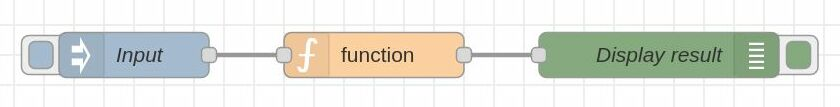
\includegraphics[width=1\textwidth]{relazione-tirocinio/Chapter-2/node-red-flows-1.jpg}
\end{figure}
Come si nota in figura appena sopra, i nodi sono dei rettangoli che hanno funzioni particolari:
\begin{itemize}
    \item Nodi input: Questi nodi emettono valori e non prendono nulla in ingresso, quindi sono utilizzati per produrre dati o iniziare dei flussi. Possono avere da 1 a n valori in uscita.
    \item Nodi intermedi: Sono nodi che hanno sia input che output. Sono utilizzati per applicare delle funzioni ai dati in ingresso, oppure il dato in ingresso viene solamente utilizzato per far iniziare una procedura intermedia. Prendono in input un solo valore e possono avere da 1 a n valori in uscita.
    \item Nodi output: Sono gli opposti dei nodi input. Non hanno valori in uscita ma solo in ingresso. Sono utilizzati per terminare un flusso, solitamente sono quindi le azioni da effettuare nel caso in cui si verificano le condizioni stabilite. Possono avere un solo valore in ingresso.
\end{itemize}
\begin{figure}[H]
\caption{Esecuzione del comando shutdown}
\label{fig:node-red-flows-example1}
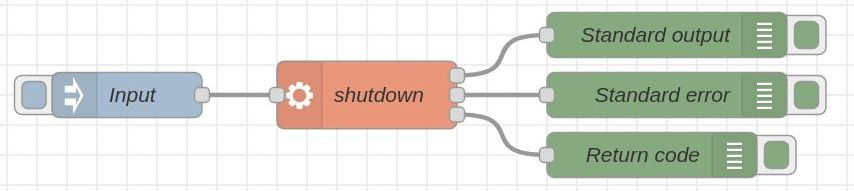
\includegraphics[width=1\textwidth]{relazione-tirocinio/Chapter-2/node-red-flows-2.jpg}
\end{figure}
Nella figura qui sopra abbiamo un altro esempio. Qui quando viene cliccato il pulsante a sinistra del nodo \textit{input}, il nodo invia in uscita un valore (in questo caso qualsiasi, ad esempio 3 o la stringa 'input') che fa eseguire il secondo nodo (di tipo \textit{intermedio}). Il nodo \textit{shutdown} esegue il comando `shutdown` e stampa nella console di debug lo stdout, stderr ed il return code.
\\
\\
Data la facilità d'uso, il grande supporto (repository con 10+K stelle su GitHub, community molto attiva e forum ufficiale), la maturità del progetto (versione 0.2 nel 2013), la facile estendibilità ed integrazione con dispositivi IoT (come appunto i sismometri), decisamente Node-RED è lo strumento più adatto per risolvere il bisogno della community SeismoCloud.
\\
\clearpage

\section{Architettura adattata a SeismoCloud}

\subsection{Come funziona Node-RED}
Può essere utilizzato in vari modi, ad esempio in locale su un computer, tramite Docker, su un dispositivo Raspberry oppure su alcuni sistemi Cloud (IBM Cloud, AWS, Microsoft Azure).
\\
Ci sono alcuni concetti di base da conoscere.
\\
Un \textbf{nodo} è il blocco costruttivo di base di un flusso. Le funzionalità dei nodi sono scatenate da eventi esterni (richieste HTTP o altro protocollo oppure un timer) o da input ricevuti da altri nodi. Processano il messaggio ricevuto oppure ne creano uno nuovo e possono inviare messaggi ai nodi successivi nel flusso. 
\\
Un \textbf{nodo di configurazione} è un tipo speciale di nodo che setta delle configurazioni utili agli altri nodi, ma non fa parte di nessun flusso. Ad esempio, i nodi \textit{MQTT-in} e \textit{MQTT-out} utilizzano il nodo di configurazione \textit{MQTT-broker} che rappresenta una connessione condivisa con un broker MQTT.
\\
Un \textbf{flusso} è rappresentato da un tab o foglio di lavoro ed è il metodo principale per organizzare il lavoro. Informalmente un flusso rappresenta un insieme di nodi connessi fra loro.
\\
Il \textbf{contesto} è il modo principale di condividere informazioni tra i nodi senza essere connessi fra loro. Ne esistono di tre tipi:
\begin{itemize}
    \item Node: Visibile solamente dal nodo che setta il valore
    \item Flow: Visibile a tutti i nodi che appartengono allo stesso flusso (o tab)
    \item Global: Visibile a tutti i nodi
\end{itemize}
Un \textbf{messaggio} è un oggetto JSON che viene passato attraverso i nodi. Di default si chiama \textit{msg} ed ha due campi: \textit{payload} e \textit{id}. 
\\
La \textbf{palette} è posizionata sulla sinistra dell'interfaccia e lista tutti i nodi presenti nel sistema. Dei nodi extra possono essere aggiunti direttamente dall'editor.
\\
Il \textbf{workspace} è lo spazio principale, dove tutti i nodi vengono posizionati in modo da creare degli automatismi.
\\
La \textbf{sidebar} è uno spazio posizionato a destra del workspace in cui ci sono degli strumenti utili, ad esempio la console di debug, l'interfaccia della configurazione dei nodi e la finestra descrittiva per ogni nodo.
\\
SCRIVI QUI
\\
Ogni flusso viene poi tradotto in codice JSON per poter essere esportato ed importato in altri ambienti.
\\
Questo semplice flusso:
\begin{figure}[H]
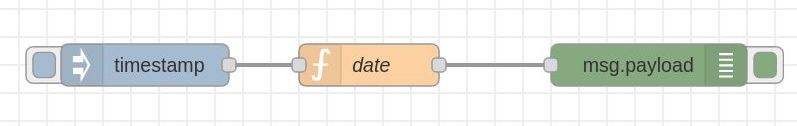
\includegraphics[width=1\textwidth]{relazione-tirocinio/Chapter-2/node-red-flows-3.jpg}
\end{figure}
Il nodo \textit{date} non è altro che un nodo function che restituisce la data:
\begin{lstlisting}[language=JavaScript]
// Create a Date object from the payload
var date = new Date(msg.payload);
// Change the payload to be a formatted Date string
msg.payload = date.toString();
// Return the message so it can be sent on
return msg;
\end{lstlisting}
Viene tradotto in JSON:
\begin{lstlisting}[language=JavaScript]
[
    {
        "id":"58ffae9d.a7005",
        "type":"debug",
        "name":"",
        "active":true,
        "complete":false,
        "x":640,"y":200,
        "wires":[]
    },
    {
        "id":"17626462.e89d9c",
        "type":"inject",
        "name":"timestamp",
        "topic":"",
        "payload":"",
        "repeat":"",
        "once":false,
        "x":240,
        "y":200,
        "wires":[["2921667d.d6de9a"]]
    },
    {
        "id":"2921667d.d6de9a",
        "type":"function",
        "name":"date",
        "func":"// Create a Date object from the payload\nvar date = new Date(msg.payload);\n// Change the payload to be a formatted Date string\nmsg.payload = date.toString();\n// Return the message so it can be sent on\nreturn msg;",
        "outputs":1,
        "x":440,
        "y":200,
        "wires":[["58ffae9d.a7005"]]
    }
]
\end{lstlisting}
\clearpage
Rimangono i gruppi trovare soluzione a ciò con nodered
\\
Utilizzo di Docker, vantaggi e svantaggi
\\
Spiegazione Architettura Node-RED
\\
Schema finale architettura
\\

\clearpage

% ======================================= CHAPTER 3 ================================================
\chapter{Implementazione delle funzionalità}

\section{Difficoltà e limiti nell'uso di Node-RED}

placeholder

\clearpage

\section{Implementazione delle funzionalità tramite nodi}

placeholder

\clearpage

\section{Ottimizzazione delle prestazioni}

placeholder

\clearpage

% ======================================= CHAPTER 4 ================================================
\chapter{Sicurezza e protezione dei dati}

\section{Sicurezza nella piattaforma Node-RED}

placeholder

\clearpage

\section{Ricerca ed analisi di vulnerabilità}

placeholder

\clearpage

\section{Risoluzione dei problemi}

placeholder

\clearpage


% ======================================= CHAPTER 5 ================================================
\chapter{Test, conclusioni e sviluppi futuri}

\section{Iterazioni dei Test}

placeholder

\clearpage

\section{Conclusioni}

placeholder

\clearpage

\section{Sviluppi futuri}

placeholder

\clearpage

\refstepcounter{chapter}

\chapter*{Ringraziamenti}

\cleardoublepage

\refstepcounter{chapter}

% ======================================= BIBLIOGRAPHY ================================================
\begin{thebibliography}{9}

\bibitem{Istituto Nazionale di Geologia e Vulcanologia}
  \textbf{Istituto Nazionale di Geologia e Vulcanologia}.
  \href{http://ingv.it}{http://ingv.it}

\bibitem{MathWorks}
  \textbf{Publish MQTT messages and subscribe to message topics}.\\
  \href{https://www.mathworks.com/help/supportpkg/raspberrypi/ref/publish-and-subscribe-to-mqtt-messages.html}{https://www.mathworks.com/help/supportpkg/raspberrypi/ref/publish-and-subscribe-to-mqtt-messages.html}

\bibitem{Node-RED Wiki}
  \textbf{Node-RED Wiki}.
  \href{https://github.com/node-red/node-red/wiki}{https://github.com/node-red/node-red/wiki}

\bibitem{Node-RED Documentation}
  \textbf{Node-RED Documentation}.
  \href{https://nodered.org/docs}{https://nodered.org/docs}

\bibitem{Docker Documentation}
  \textbf{Docker Documentation}.
  \href{https://docs.docker.com/}{https://docs.docker.com/}

\end{thebibliography}

\end{document}